\documentclass[12pt]{paper}
\usepackage{epsfig}
\usepackage{latexsym}
\usepackage{amssymb}
\usepackage[english]{babel}
\usepackage{amsmath}
\usepackage{enumerate}
   
\newcommand{\beq}{\begin{equation}}
\newcommand{\eeq}{\end{equation}}
\newcommand{\bga}{\begin{gathered}}
\newcommand{\ega}{\end{gathered}}
% Margins
\topmargin=-0.45in
\evensidemargin=0in
\oddsidemargin=0in
\textwidth=6.5in
\textheight=9.0in
\headsep=0.25in 

\title{Detectability of high-z MFs with radio arrays}
%\author{}

\begin{document}
\maketitle

\section{Basic definitions}

The redshifted 21-cm signal is commonly represented using four equivalent quantities encoding the specific intensity (with respect to the CMB background): intensity as a function of the observed location in physical space $I(\vec{r})$, its Fourier transform $\widetilde{I}(\vec{k})$, and the scaled versions of these two functions, in sky and frequency coordinates: $\mathcal{I}(\theta_x, \theta_y, f)$, and $\widetilde{\mathcal{I}}(u,v,\eta)$.

Vector $\vec{k}$ (in comoving Mpc$^{-1}$) is a Fourier dual of $\vec{r}$ (in comoving Mpc), and likewise, $(\theta_x[rad], \theta_y[rad], f[Hz])$ are duals of $(u[rad^{-1}], v[rad^{-1}], \eta[sec])$. These two sets of coordinates are related through linear transformations in the following way
\begin{equation}
\begin{gathered}
\theta_x = \frac{r_x}{D_M(z)}, \hspace{0.5in} u = \frac{k_xD_M(z)}{2\pi},\\
\theta_y = \frac{r_y}{D_M(z)}, \hspace{0.5in} v = \frac{k_yD_M(z)}{2\pi},\\
f = \frac{H(z)f_{21,0}}{c(1+z)^2} r_z, \hspace{0.5in} \eta = \frac{c(1+z)^2}{2\pi H(z)f_{21,0}}k_z,
\end{gathered}
\label{eq:fourier_duals}
\end{equation} 
where $f_{21,0}$ is the 21-cm frequency in the rest frame, $H(z)$ iz the Hubble parameter, $D_M(z)$ is the comoving distance in transverse direction, and z is the reference redshift in the middle of the observed data cube (where $r_z$ and $f$ intervals are evaluated). Note that the conditions of type $2\pi\theta_xu = r_xk_x$ are saticefied\footnote{The factor of $2\pi$ just comes from the Fourier-transform conventions in Eqs.~\ref{eq:mathcal_I_tildeI} and \ref{eq:mathcal_tildeI_I}.}.

Now we can establish conventions for the Fourier transforms that relate the four intensity representation as follows
\beq
I(\vec{r}) = \int\widetilde{I}(\vec{k})e^{i\vec{k} \cdot \vec{r}}d^3\vec{k},
\label{eq:I_tildeI}
\eeq
\beq
\widetilde{I}(\vec{k}) = \frac{1}{(2\pi)^3}\int{I}(\vec{k})e^{-i\vec{k} \cdot \vec{r}}d^3\vec{r},
\label{eq:tildeI_I}
\eeq
\beq
\mathcal{I}(\theta_x,\theta_y,f) = \int\int\int\widetilde{\mathcal{I}}(u,v,\eta)e^{2\pi i(u\theta_x + v\theta_y+\eta f)}dudvd\eta,
\label{eq:mathcal_I_tildeI}
\eeq
\beq
\widetilde{\mathcal{I}}(u,v,\eta) = \int\int\int{\mathcal{I}}(\theta_x,\theta_y,f)e^{-2\pi i(u\theta_x + v\theta_y+\eta f)}d\theta_xd\theta_ydf,
\label{eq:mathcal_tildeI_I}
\eeq
such that the following scaling relation is saticefied
\begin{equation}
\widetilde{I}(\vec{k}) = \frac{H(z)f_{21,0}}{c(1+z)^2D_M(z)^2}\widetilde{\mathcal{I}}(u,v,\eta),
\label{eq_tilde_I_vs_Ik_scaling}
\end{equation}
where the proportionallity factor between these two functions is a Jacobian $\frac{d\theta_xd\theta_ydf}{dr_xdr_ydr_z}$ (this scaling was obtained by substituting Eq.~\ref{eq:fourier_duals} into Eq.~\ref{eq:mathcal_tildeI_I}, and comparing the result to Eq.~\ref{eq:tildeI_I}). Note also that there is no scaling between $I$ and $\mathcal{I}$---they are the same function, up to change of variables.

Finally, since radio interferometers measure visibilities, we define the visibility for a pair of antennae as a Fourier-transform in frequency-coordinate only of the $uv$-plane specific intensity,
\beq
\mathcal{\widetilde{I}}(u,v,\eta) = \int V(u,v,f)e^{-2\pi f\eta}df,
\label{eq:visibility}
\eeq
where $f$ is a discrete variable such that $f_\text{max}-f_\text{min}=\Delta f$ is the bandwidth of the observed data cube centered on $z$ (see also Appendix \ref{app_Vrms}).
%%%%%%%%%%%%%%%%%%%
\section{Power spectra definitions}

We want to derive an expression for the power spectrum of noise intensity (including instrument noise, and noise from the sky) in $\vec{k}$ space. This power spectrum is given by
\beq
\langle \widetilde{I}(\vec{k})\widetilde{I}^*(\vec{k}')\rangle = (2\pi)^3P_{\widetilde{I}}\delta(\vec{k}-\vec{k}').
\label{eq_tildeI_power}
\eeq

On the other hand, the measurable quantity---the visibility---is a complex Gaussian variable with a zero mean, whose noise-induced component has a variance of\footnote{See Appendix for a derivation of $V_\text{rms}$.}
\beq
\langle V(\vec{u},f)V(\vec{u}',f')^*\rangle = \left(\frac{2k_BT_\text{sys}}{A_e\sqrt{\Delta f t_1}}\right)^2 \delta(\vec{u}-\vec{u}')\delta_{ff'},
\label{eq_Vrms}
\eeq 
where $t_1$ is the total time a single baseline spent observing an element at the position $\vec u \equiv(u,v)$ in the $uv$ plane. 

%%%%%%%%%%%%%%%%%%%
\section{From visibility to $P^N(\vec k)$}

The next step is to combine Eqs.~\ref{eq:visibility}, and \ref{eq_Vrms}, and take ensamble average to get
\beq
\bga
\langle\widetilde{\mathcal{I}}(u,v,\eta) \widetilde{\mathcal{I}}^*(u',v',\eta')\rangle =  \int\int\langle V(u,v,f)V^*(u',v',f')\rangle e^{2\pi i(f'\eta'-f\eta)}dfdf'\\
= \frac{1}{t_1}\left(\frac{2k_BT_\text{sys}}{A_e}\right)^2 \delta(\vec{u}-\vec{u}')\delta(\eta-\eta'),
\ega
\label{eq:mathcal_power_Vrms}
\eeq 
where 
\beq
\int e^{2\pi i f(\eta-\eta')}df =\delta(\eta-\eta'),
\eeq
is the periodic delta-function on the $t_1$ interval, and $D_\text{band}$ is the total bandwidth of this data cube centered on $z$.  

As the final step, we need to take into account the scaling relation of Eq.~\ref{eq_tilde_I_vs_Ik_scaling} and substitute it on the LHS of the above equation, and then introduce the power spectrum of Eq.~\ref{eq_tildeI_power}. In addition, keeping in mind the property of the delta-function that $\delta(ax)=\frac{1}{a}\delta(x)$, we can substitute the relations between variables in Eq.~\ref{eq:fourier_duals} to cancel the delta functions in Eq.~\ref{eq:mathcal_power_Vrms}. We thus arrive at the following expression for the noise power spectrum, per $\vec k$ mode, per baseline,
\beq
P_1^N(\vec k) = \frac{1}{t_1}\frac{c(1+z)^2D_M^2(z)}{H(z)f_{21,0}}\left(\frac{2k_BT_\text{sys}}{A_e}\right)^2 .
\label{eq:Pnoise_1mode}
\eeq

Note now that the computation of $t_1$ from the total duration of the survey  $t_\text{obs}$ will depend on the type of the experiment.\footnote{Also note that we are not accounting for the fact that a given patch of the sky is only visible for a part of a day from a given location, so $t_\text{obs}$ is actually the survey duration, times a factor of a few or less.}  For a small beam size (much smaller than $\Omega_\text{survey}$), where telescopes scan the sky one beam width at a time, like for the case of radio dishes, $t_1$ is the total time spent observing a given $uv$ element of size corresponding to the beam $\Omega_\text{beam}=\lambda^2/A_e$, and is obtained by multiplying  $t_\text{obs}$ by the ratio of the solid angle of the survey and the solid angle of the beam, $\Omega_\text{survey}/\Omega_\text{beam}$. However, in the case of simple dipole antennas, the beam is greater or equal to the survey angular size, and in this case $t_1$ just equals $t_\text{obs}$.

The last step is to get from Eq.~\ref{eq:Pnoise_1mode} to the expression for the noise power spectrum that corresponds to the observation with all the available baselines. To do that, we need to incorporate the knowledge about the array configuration and the coverage of the $uv$ plane. In other words, we need to divide the expression in Eq.~\ref{eq:Pnoise_1mode} by the number of baselines that see a given mode $\vec k$ at any given time $n_\text{base}(\vec k)$ (for a discussion of the $uv$ coverage, see the following section). The final result for the noise power spectrum per mode $\vec k$ in the intensity units is then
\beq
P^N(\vec k) = \frac{1}{t_\text{1}}\frac{c(1+z)^2D_M^2(z)}{H(z)f_{21,0}}\frac{\left(2k_BT_\text{sys}\right)^2}{A_e^2n_\text{base}(\vec k)},
\label{eq:Pnoise_Jy}
\eeq
and in temperature units
\beq
P^N(\vec k) = \frac{\lambda^4}{t_\text{1}}\frac{c(1+z)^2D_M^2(z)}{H(z)f_{21,0}}\frac{T_\text{sys}^2}{A_e^2n_\text{base}(\vec k)}.
\label{eq:Pnoise_K}
\eeq
Ta-dah!
%%%%%%%%%%%%%%%%%%%
\section{The UV Coverage}
\label{sec:uv_coverage}

Total number of baselines that can observe mode $\vec k$, $n_\text{base}(\vec k)$, is related to the (unitless) number density of baselines per element $dudv$, $n(u,v)$, as
\beq
n_\text{base}(\vec k) = \frac{n(u,v)}{\Omega_\text{beam}},
\label{eq:nuv_nk}
\eeq
where $\frac{1}{\Omega_\text{beam}}$ represents an element in the $uv$ plane, and the number density integrates to the total number of baselines $N_\text{base}$ as 
\beq
N_\text{base}=\frac{1}{2}N_\text{ant}(N_\text{ant}+1) = \int_\text{half} n(u,v)dudv,
\label{eq:nk}
\eeq
where $N_\text{ant}$ is the number of antennas in the array, and the integration is done on the half of the $uv$ plane\footnote{This is because the visibility has the following property $V(u,v,f)=V^*(-u,-v,f)$, and only half the plane contains independent samples.}.

Let us now derive $n(\vec k)$ for a specific array configuration that is of particualr interest to cosmology\footnote{Note also that we assume that the array consists of many antennas, so that time-dependence of $n(u,v)$ is negligible; if this is not the case, one should compute its time average to account for Earth's rotation.} ---a tightly packed array of simple dipole antennas, tiling a squared-surface of the area $(\Delta L)^2$ with a filling fraction close to one (see Figure \ref{fig:nk_fft}).\footnote{This assumes a design such as the FFT telescope described in Tegmark and Zaldarriaga (2009).} In this case, the beam is close to the size of the entire survey and coveres 1 sr, the affective area of a single dipole is $A_e = \lambda^2$, and the effective number of antennas is then $N_\text{ant} = \frac{(\Delta L)^2}{\lambda^2}$.

A uniform tiling of a $(\Delta L)^2$ surface with dipoles then results in the following number density of baselines per $uv$ element
\beq
n(u,v) = (\frac{\Delta L}{\lambda} - u)(\frac{\Delta L}{\lambda} - v).
\label{eq:nuv_fftt}
\eeq
After substituting the relation between $\vec k=(k,\theta_k,\phi_k)$ and $(u,v)$, 
\beq
\bga
u_\perp \equiv \frac{D_A(z)}{2\pi}k\sin\theta_k,\\
u = u_\perp \cos\phi_k,\\
v = u_\perp \sin\phi_k,
\ega
\label{eq:k_uv}
\eeq
the corresponsing number of baselines observing a given $\vec k$ at a given time where azimuthal angle of the mode in the frame where $\widehat n$ is the vertical axis is $\phi_k$ is then
\beq
n_\text{base}(\vec k) = (\frac{\Delta L}{\lambda} - \frac{D_A(z)}{2\pi}k\sin\theta_k\cos\phi_k)(\frac{\Delta L}{\lambda} - \frac{D_A(z)}{2\pi}k\sin\theta_k\sin\phi_k).
\label{eq:nk_fftt}
\eeq
We will use a $\phi_k$-averaged version of this quantity (between $0$ and $\pi/2$ only, due to the four-fold symmetry of the experimental setup of a square of dipoles), to account for the rotation of the baselines with respect to the modes,
\beq
\langle n_\text{base}(\vec k) \rangle_{\phi_k}= \left(\frac{\Delta L}{\lambda}\right)^2 -\frac{4}{\pi}\frac{\Delta L}{\lambda}\frac{D_A(z)}{2\pi}k\sin\theta_k + \left(\frac{D_A(z)}{2\pi}k\sin\theta_k\right)^2.
\label{eq:nk_fftt_mean}
\eeq
%%%%%%%%%%%%%%%%%%%
\section{MVQ estimator for a uniform field}
\label{sec:B_estimator}

We will now derive an unbiased minimum-variance quadratic estimator $\widehat B$ for a uniform magnetic field (MF) $\vec B$, following a similar CMB formalism. We start by noting that the redshifted 21-cm brightness temperature contains contribution from the noise, and the signal, where the signal is generated both by the 21-cm signal with no magnetic field (null-case signal), and by $\vec B$, such that
\beq
\bga
T(\vec k) = T_N(\vec k) + T_S(\vec k),\\
T_S(\vec k) = T_{S,0}(\vec k) + B\frac{\partial T_S(\vec k)}{\partial B}\bigg|_{B=0},
\ega
\label{eq:Ttot}
\eeq
where the magnitude of the field $B$ is a small expansion parameter. The derivative in the above equation is evaluated at $B=0$, and similarly for the signal $T_{S,0}$ in the null case.  We can now compute the following expectation value
\beq
\langle T(\vec k)T^*(\vec k')\rangle = P_\text{null}(\vec k)(2\pi)^3\delta(\vec k-\vec k') + \langle T_{S,0}(\vec k)B\frac{\partial T_S^*(\vec k')}{\partial B}\bigg|_{B=0}\rangle + \langle T_{S,0}^*(\vec k')B\frac{\partial T_S(\vec k)}{\partial B}\bigg|_{B=0}\rangle
\label{eq:TT_step1}
\eeq
where we introduced notation for the power spectrum in the null case,
\beq
P_\text{null}(\vec k) \equiv P^N(\vec k) + P_0^S(\vec k),
\label{eq:Pnull}
\eeq
such that $P^S_0$ represents the 21-cm power spectrum in the absence of MFs. We have also assumed that the signal and the noise are uncorrelated, and kept only terms linear in $B$. To expand the RHS of Eq.~\ref{eq:TT_step1} further, we first note that the only Gaussian random field the signal temperature is proportional to is the density fluctuation $\delta$, with the proportionality being the transfer funtion $G$,
\beq
\bga
T_S(\vec k) = G(\hat k)\delta(k),\\
T_{S,0}(\vec k) = G(\hat k,B=0)\delta(k),
\ega
\label{eq:def_G}
\eeq
where $\hat k$ is a unit vector in the direction of $\vec k$. In this case, we note that
\beq
\frac{\partial T_S(\vec k)}{\partial B} =  \delta(k)\frac{\partial G(\vec k)}{\partial B},
\label{eq:dTdB_dGdB}
\eeq
where the derivative will be evaluated at $B=0$. Eq.~\ref{eq:TT_step1} now becomes
\beq
\langle T(\vec k)T^*(\vec k')\rangle = \left(P_\text{null}(\vec k) + 2BP_{\delta}(\vec k)Re\left[G^*(\vec k,B=0)\frac{\partial G(\vec k)}{\partial B}\bigg|_{B=0}\right]\right) (2\pi)^3\delta(\vec k-\vec k').
\label{eq:TT_step2}
\eeq
Note here that the delta function evaluates to
\beq
\delta(\vec k-\vec k') = \frac{V}{(2\pi)^3},\hspace{0.2in} \text{for }\vec k = \vec k',
\label{eq:delta_kk}
\eeq
where $V$ is the space volume of the survey, in our case. 

The next step is to note that we observe only one universe, so the measured proxy for the ensamble average of Eq.~\ref{eq:TT_step2} will be just the product $T(\vec k)T^*(\vec k)$.  Using this fact and Eq.~\ref{eq:delta_kk}, and inverting Eq.~\ref{eq:TT_step2} gives an estimate for $B$ from a single $\vec k$-mode measurement,
\beq
\widehat B_{\vec k} = \frac{\frac{1}{V}T(\vec k)T^*(\vec k) - P_\text{null}(\vec k)}{2P_{\delta}(\vec k)Re\left[G^*(\vec k,B=0)\frac{\partial G(\vec k)}{\partial B}\bigg|_{B=0}\right]}.
\label{eq:hatBk}
\eeq 
This estimator is unbiased, $\langle \widehat B_{\vec k}\rangle=0$, and the above expression can be used to calculate its covariance, from
\beq
C_{\vec k,\vec k'} \equiv \langle \widehat B_{\vec k}\widehat B^*_{\vec k'}\rangle = 
\frac{\left\langle\left(\frac{1}{V}T(\vec k)T^*(\vec k) - P_\text{null}(\vec k)\right)\left(\frac{1}{V}T^*(\vec k')T(\vec k') - P_\text{null}(\vec k')\right)\right\rangle}{4P_{\delta}(\vec k)P_{\delta}(\vec k')Re\left[G^*(\vec k)\frac{\partial G(\vec k)}{\partial B}\right]Re\left[G(\vec k')\frac{\partial G^*(\vec k')}{\partial B}\right]},
\label{eq:mean_BB}
\eeq
where all derivatives and $G$ are evaluated at $B=0$, following, as usual, the null assumption. For simplicity, from now on, we drop the explicit notation for $B=0$ but retain the null assumption in the entire derivation.  The expectation value in the above equation involves temperature four-point correlation. If we enumerate factors of ``$T$'' in this correlation as $\langle 1\text{ }2\text{ }3\text{ }4\rangle$, the expansion of this correlation of four Gaussian random variables can be represented as a sum of the following contractions: $\langle T(\vec k)T^*(\vec k)T^*(\vec k')T(\vec k') \rangle=\langle1\text{ }2\rangle\langle3\text{ }4\rangle+
\langle1\text{ }4\rangle\langle2\text{ }3\rangle+\langle1\text{ }3\rangle\langle2\text{ }4\rangle$. Keeping this order of summands, the correlation becomes
\beq
\langle T(\vec k)T^*(\vec k)T^*(\vec k')T(\vec k') \rangle = V^2P_\text{null}(\vec k)^2\left( 1+\delta_{\vec k,\vec k'}+\delta_{\vec k,-\vec k'}\right)
\label{eq:TTTT_expansion}
\eeq
where we used Eq.~\ref{eq:delta_kk}, and the relation between delta function and Kronecker delta,
\beq
\delta_{\vec k,\vec k'} = \frac{(2\pi)^3}{V}\delta(\vec k-\vec k').
\label{eq:deltas}
\eeq
The rest of the terms in Eq.~\ref{eq:mean_BB} are of the form
\beq
\bga
\frac{1}{V}\langle T(\vec k)T^*(\vec k)\rangle P_\text{null}(\vec k') =  P_\text{null}(\vec k)P_\text{null}(\vec k').
\ega
\label{eq:BB_crossterms}
\eeq
Finally, substituting Eqs.~\ref{eq:TTTT_expansion}, \ref{eq:BB_crossterms}, and \ref{eq:deltas}, into Eq.~\ref{eq:mean_BB}, we get the following expression for the covariance
\beq
\langle \widehat B_{\vec k}\widehat B^*_{\vec k'}\rangle = \frac{P_\text{null}^2(\vec k)\left(\delta_{\vec k,\vec k'}  + \delta_{\vec k,-\vec k'} \right)}{\left(2P_{\delta}(\vec k)Re\left[G^*(\vec k)\frac{\partial G(\vec k)}{\partial B}\right]\right)^2},
\label{eq:B_covariance}
\eeq
where the variance $\sigma^2_{\vec k}\equiv\langle \widehat B_{\vec k}\widehat B^*_{\vec k}\rangle $ represents diagonal elements of the covariance matrix.

This covariance matrix is singular, and the only non-vanishing entries are those relating the same mode with itself (or to the same mode in the opposite direction), which is a consequence of the reality of the temperature field, and the isotropy of space in the null-assumption case. The usual expression for a minimum-variance estimator,
\beq
\widehat B = \frac{\sum_{\vec k, \vec k'}C^{-1}_{\vec k, \vec k'}\widehat B_{\vec k}}{\sum_{\vec k, \vec k'}C^{-1}_{\vec k, \vec k'}},
\label{eq:B_mve}
\eeq
in this case reduces to 
\beq
\bga
\widehat B = \frac{1}{2}\frac{\sum_{\vec k}\frac{\widehat B_{\vec k}}{\sigma^2_{{\vec k}}}}{\sum_{\vec k}\frac{1}{\sigma^2_{\vec k}}},
\ega
\label{eq:B_mve}
\eeq
where the factor of $\frac{1}{2}$ comes from the two Kronecker deltas in Eq.~\ref{eq:B_covariance}. The final expression for the estimator is then
\beq
\bga
\widehat B = \frac{\sum_{\vec k}\frac{\frac{1}{V}T(\vec k)T^*(\vec k) - P_\text{null}(\vec k)}{P_\text{null}^2(\vec k)}P_{\delta}(\vec k)Re\left[G^*(\vec k)\frac{\partial G(\vec k)}{\partial B}\right]}{{\sum_{\vec k}\left(\frac{2P_{\delta}(\vec k)Re\left[G^*(\vec k)\frac{\partial G(\vec k)}{\partial B}\right]}{P_\text{null}(\vec k)}\right)^2}},
\ega
\label{eq:B_estimator}
\eeq
Note at the end that the expression in the denominator is exactly the expression for the integrand for the inverse variance of the Fisher forecast, as expected. 
 %%%%%%%%%%%%%%%%%%%%%%%%
\section{Fisher Analysis}
\label{sec:fisher}

We will first discuss the unsatured case, where the strength of $\vec B$ produces less than 1 rad of precession at all z of interest, and then move on to discussing detectability in the saturated case, where $B$ is strong in this sense.

If an experiment measures redshifted 21-cm brightness-temperature power spectrum $P(k,\theta_k,\phi_k)$, which is a function of a parameter $B$ (in this case, the strength of a uniform MF that evolves as $B=B_0(1+z)^2$), then this experiment's sensitivity to recovering $B$ is given by the Fisher matrix, which combines measurements at every $(k,\theta_k,\phi_k)$ mode,
\begin{equation}
\begin{gathered}
\sigma_{B_0}^{-2}(z) = \int dV_\mathrm{patch}(z)
\frac{k^2dk d\phi_k\sin \theta_kd\theta_k}{(2\pi)^3}\left(  \frac{\frac{\partial P_S}{\partial B}}{P_N + P_S }\right)^2 \\
=\int dV_\mathrm{patch}(z)
\frac{k^2dk d\phi_k\sin \theta_kd\theta_k}{2(2\pi)^3}\left( \frac{2P_\delta(k,z)G(B=0,\theta_k,\phi_k)\frac{\partial G}{\partial B}(\theta_k, \phi_k,z)\bigg|_{B=0}}{P_N(k,\theta_k) + P_\delta(k,z)G^2(B=0,\theta_k,\phi_k)} \right)^2,
\end{gathered}
\label{eq:fisher_patch}
\end{equation}
where $V_\mathrm{patch}$ is the comoving volume of the survey, such that
\beq
dV_\mathrm{patch} = \frac{c}{H(z)}D_A^2\Omega_\mathrm{survey}dz.
\label{eq:dVpatch}
\eeq
Note that we operate under the null assumtion of small $B$, so every summand in the above equation is evaluated for a fiducial case of $B=0$. In this case, the above expression can be used to compute magnitude of $B$ detectable at 1-$\sigma$ level for a given noise level (and cosmology). The power spectrum of the 21-cm signal is in the denominator of the summands in order to account for sample variance. In our case, it is computed for a given cosmology, as
\begin{equation}
P_S = G^2(\theta_k, \phi_k) P_\delta (k),
\label{eq:PS}
\end{equation}
where $P_\delta$ is the power spectrum of density fluctuations at a given redshift, for a given cosmology, and $G$ is the transfer function (a function of $B$ computed from microphysical calculations of Paper I).\footnote{Note here that we do not take the average of the noise over $\phi_k$, because we are interested in reconstructing the sensitivity of a given $(B,\theta_B,\phi_B)$. }
The integration limits in Eq.~\ref{eq:fisher_patch} are: $\phi_k\in[0,2\pi]$; $\theta_k\in [0,\pi]$; and $k\in[2\pi u_\mathrm{min}/(d_A\sin\theta_k),2\pi u_\mathrm{max}/(d_A\sin\theta_k)]$, where $u_\mathrm{min, max}=\frac{L_\text{min, max}}{\lambda}$ correspond to the maximum and minimum baseline, respectively.

Before going on to the saturated case, let us note that the integral in Eq.~\ref{eq:fisher_patch} is performed on a small, approximately flat, patch of the sky. If the survey area is big enough that this approximation does not hold in the entire survey patch, then this integral should be performed on small parts of the survey, and the results added in quadriture to obrain the sensitivity of the entire survey. This will then account for the change in the angle that a uniform field $\vec B$ makes with a line of sight (LOS), as the LOS moves through a large survey area, and the total sensitivity is given with
\beq
\sigma^{-2}_{B_0,\text{ survey}} = \frac{\sigma^{-2}_{B_0,\text{ patch}}}{\Omega_\text{patch}} \int_0^{\theta_\text{survey}}\int_{0}^{2\pi} \cos^2 \theta d\theta d\phi 
= \frac{\pi}{\Omega_\text{patch}} \left(\theta_\text{survey} + \cos \theta_\text{survey} \sin \theta_\text{survey}\right).
\label{eq:sigma_sum_survey}
\eeq

For the saturated case, we are unable to measure the exact magnitude of $B$, but a slightly different inquiry becomes interesting. Namely, it is useful to know how sensitive are future experiments to distinguishing staturated case from zero MF. To make a forecast for this question, let us write the signal power spectrum as a sum of the contributions from very weak field (a.k.a. $B=0$), and very strong field (denoted as infinity), 
\beq
P = (1-\xi)P\bigg|_{B\to 0} + \xi P\bigg|_{B\to \infty},
\label{eq:saturated_P}
\eeq
where we have not explicitly written the indicies and dependencies, to maximize clarity of the equation. We can then perform the standard Fisher analysis, completely analogous to the unsaturated case, in order to understand constraints on parameter $\xi$. In this case, $\sigma_\xi$ would give a 1-$\sigma$ sensitivity to detecting the maximum change in $G$, due to the rise to the saturation ceiling (see Figure \ref{fig:B0zeta_vs_deltas}). 

%%%%%%%%%%%%%%%%%%%
\section{MVQ estimator for a stochastic field}

We now wish to compute the noise level for the measurement of the power spectrum of a stochastic magnetic field. Following the MVQ estimator derivation of \S\ref{sec:B_estimator}, and focusing on a single component $B_i$ of $B$ at a time, we start with
\beq
T(\vec x) = T_0(\vec x) + B_i(\vec x)\frac{\partial T_0}{\partial B_i}(\vec x),
\eeq
where the subscript $0$ indicates no magnetic field (null assumption). We then transition to Fourier space,
\beq
\bga
T(\vec k) = T_0(\vec k) + \int d\vec x e^{-i\vec k \cdot \vec x} B_i(\vec x) \frac{\partial T_0}{\partial B_i}(\vec x)
= T_0(\vec k) + \frac{1}{(2\pi)^3}\int d\vec k_1B_i(\vec k_1) \frac{\partial T_0}{\partial B_i}(\vec k-\vec k_1),
\ega
\eeq
where $k_1$ is the integration variable, and the last step used the convolution theorem. It further follows
\beq
\bga
\left < T(\vec k)T^*(\vec k')\right > = \left < T_0(\vec k)T_0^*(\vec k')\right >\\
+ \left <T_0^*(\vec k')\frac{1}{(2\pi)^3}\int d\vec k_1 B_i(\vec k_1) \frac{\partial T_0}{\partial B_i}(\vec k-\vec k_1)\right > + \left <T_0(\vec k)\frac{1}{(2\pi)^3}\int d\vec k_1 B_i^*(\vec k_1) \left(\frac{\partial T_0}{\partial B_i}(\vec k'-\vec k_1)\right)^*\right >, 
\ega
\eeq
to first order in $B_i$. Now, let us remember that
\beq
\bga
T(\vec k) = G(\vec k) \delta(\vec k),\\
\frac{\partial T}{\partial B_i}(\vec k) = \frac{\partial G}{\partial B_i}(\vec k) \delta(\vec k),
\ega
\eeq
and that
\beq
\bga
\left<\delta(\vec k)\delta^*(\vec k')\right> \equiv (2\pi)^3 \delta_D(\vec k-\vec k') P_\delta(\vec k),\\
\left<T_0(\vec k)T_0^*(\vec k')\right> \equiv (2\pi)^3 \delta_D(\vec k-\vec k') G^2_0(\vec k)P_\delta(\vec k),
\ega
\eeq
in a statistically isotropic and homogenous universe. The notation $\delta_D(\vec k-\vec k')$ stands for the Dirac delta function, related to the Kronecker delta as $(2\pi)^3 \delta_D(\vec k-\vec k') = V \delta_{\vec k\vec k'}$, in a finite volume. \footnote{Delta functions are not to be confused with the density perturbation Fourier mode $\delta(\vec k)$.} Also note that $\delta_{\vec k,\vec k'}= (2\pi)^3/V$, for $\vec k = \vec k'$. From this, the Fourier-space 2-point correlation for the brightness temperature becomes\footnote{Notice that we had to transition from Dirac to Kronecked delta in order to perform the integrals within the brakets, which is where the volume V factor will come from.}
\beq
\bga
\left< T(\vec k)T^*(\vec k')\right> = (2\pi)^3\delta_D(\vec k - \vec k')  G_0^2(\vec k)P_\delta(\vec k) \\
+B_i(\vec k - \vec k')\left[ P_\delta(\vec k')G_0^*(\vec k')\frac{\partial G_0}{\partial B_i}(\vec k') - P_\delta(\vec k)G_0(\vec k)\frac{\partial G_0^*}{\partial B_i}(\vec k)\right],
\ega
\eeq
where we used the reality of the $B_i$ field, $B_i^*(-\vec k) = -B_i(\vec k)$.
Now, if we wish to estimate $B_i(\vec K\equiv\vec k-\vec k')$ only from $\vec k,\vec k'$ pair of modes, we get
\beq
\widehat B_i^{\vec k\vec k'}(\vec K) = \frac{T(\vec k)T^*(\vec k')}{P_\delta(\vec k')G_0^*(\vec k')\frac{\partial G_0}{\partial B_i}(\vec k') - P_\delta(\vec k)G_0(\vec k)\frac{\partial G_0^*}{\partial B_i}(\vec k)},
\label{eq:Bkkp_estimator}
\eeq
where the hat sign indicates an estimator. Note that we now only focus on terms $\vec K\ne0$ ($\vec k \ne\vec k'$).
The variance of this estimator (evaluated under the null assumption) is 
\beq
\bga
\left< \widehat B_i^{\vec k\vec k'}(\vec K)\left(\widehat B_i^{\vec k\vec k'}(\vec K')\right)^*\right> = \\
\frac{\left<  T(\vec k)T^*(\vec k')T^*(\vec k)T(\vec k') \right>}{\left(P_\delta(\vec k')G_0^*(\vec k')\frac{\partial G_0}{\partial B_i}(\vec k') - P_\delta(\vec k)G_0(\vec k)\frac{\partial G_0^*}{\partial B_i}(\vec k)\right)\left(P_\delta(\vec k')G_0(\vec k')\frac{\partial G_0^*}{\partial B_i}(\vec k') - P_\delta(\vec k)G_0^*(\vec k)\frac{\partial G_0}{\partial B_i}(\vec k)\right)}.
\ega
\label{eq:Bkkp_var}
\eeq

Finally, using Eqs.~(\ref{eq:Bkkp_estimator}) and (\ref{eq:Bkkp_var}), we can derive the MVQ estimator for the mode $\vec K$ of $B_i$, in the usual way (by combining the individual $\widehat B_i^{\vec k\vec k'}(\vec K)$ estimates with inverse-variance weights, and normalizing appropriately). The noise power spectrum is then the variance of such an estimator,
\beq
\bga
(2\pi)^3\delta_D(\vec K - \vec K') P^N_{B_i}(\vec K) \equiv \left< \widehat B_i(\vec K)\widehat B_i(\vec K')^*\right>\\
= \left( \sum_{\vec k} \frac{1}{2}\frac{\left|P_\delta(\vec k')G_0^*(\vec k')\frac{\partial G_0}{\partial B_i}(\vec k') - P_\delta(\vec k)G_0(\vec k)\frac{\partial G_0^*}{\partial B_i}(\vec k)\right|^2}{V^2\left(G^2_0(\vec k)P_\delta(\vec k) + P^N(\vec k)\right)\left(G^2_0(\vec k')P_\delta(\vec k') + P^N(\vec k')\right) } \right)^{-1},
\ega
\label{eq:NK1}
\eeq
with the restriction $\vec K=\vec k-\vec k'$, and where the factor of $1/2$ serves to avoid double-counting mode pairs. As before, $P^N$ is given by Eq.~(\ref{eq:Pnoise_K}). If we limit ourselves to the diagonal terms only where $\vec K=\vec K'$, then the LHS becomes $V P^N_{B_i}(\vec K)$. Furthermore, to transition from a sum over $\vec k$ modes to an integral, we can use $\sum_{\vec k} \to V\int d\vec k /(2\pi)^3$. The resulting expression for the noise power spectrum is then
\beq
\bga
P^N_{B_i}(\vec K) = \left(\frac{1}{2}\int d{\vec k} \frac{\left|P_\delta(\vec k')G_0^*(\vec k')\frac{\partial G_0}{\partial B_i}(\vec k') - P_\delta(\vec k)G_0(\vec k)\frac{\partial G_0^*}{\partial B_i}(\vec k)\right|^2}{\left(G^2_0(\vec k)P_\delta(\vec k) + P^N(\vec k)\right)\left(G^2_0(\vec k')P_\delta(\vec k') + P^N(\vec k')\right) } \right)^{-1},
\ega
\label{eq:NK}
\eeq
Note that only the components of $\vec B$ in the plane of the sky have an effect of the observed brightness temperature, and so the above expression holds for those components. The noise in these two components is not correlated, and the noise in the direction along the line of sight can be considered infinite.
%%%%%%%%%%%%%%%%%%%
\section{SNR calculation}
\label{sec:snr}

We will here only focus on the calculation of SNR for detecting a particular model of MF power spectrum, for the case where most of the signal comes from the largest modes (smallest $\vec K$'s). In this (squeezed) limit, $\vec K \ll \vec k$ and thus $\vec k \approx \vec k'$, such that the noise power spectrum of Eq.~(\ref{eq:NK}) becomes white noise (independent on $\vec K$).  If we further denote pixels with Greek indicies, and, as before, retain Roman indicies for components of $\vec B$, then the pixel-noise variance for measuring a single mode $\vec K$ of $B_i$ component is $\sigma_{B_i}^2 \equiv P^N_{B_i}(z)/V_\text{voxel}$, where $V_\text{voxel}$ is volume of a survey voxel (3d pixel). The model for the power spectrum is defined through
\beq
(2\pi)^3\delta_D(\vec K - \vec K') P_{B_iB_j}(\vec K) = \left<B_i^*(\vec K) B_j(\vec K')\right>,
\label{eq:Pbb}
\eeq
which relates to the variance in the transverse component $P_B(\vec K)$ as
\beq
P_{B_iB_j}(\vec K) = (\delta_{ij} - \widehat K_i \widehat K_j) P_B(\vec K),
\label{eq:Pbb_Pb}
\eeq
where $\widehat K_{i/j}$ is a unit vector along the direction of a $B_{i/j}$ component.
In this discussion, as a model example, we consider a scale-independent power spectrum, were
\beq
P_{B}(\vec K) = A_0/K^3,
\label{eq:SI}
\eeq
and the amplitude $A_0$ is a free parameter in units of Gauss.

To compute SNR for measuring the amplitude of an arbitrary power-spectrum model in a given redshift slice $z$, we have to perform a sum over all voxels in the survey volume at that $z$. The general expression for SNR is
\beq
\text{SNR}^2 = \frac{1}{2} Tr \left( N^{-1}SN^{-1}S\right),
\label{eq:snr_general}
\eeq
where S is the signal matrix, N is the noise matrix. In our case, these matrices are $3N_\text{voxels}\times 3N_\text{voxels}$ (assuming there are $N_\text{voxels}$ voxels in the entire survey, and that there are 3 components of $vec B$). In the null case, voxels are independent, and so the noise matrix is diagonal, and the signal is the 3d power spectrum of the vector field $\vec B$. For a single redshift slice, this evaluates to 
\beq
\text{SNR}^2 (z)= \frac{1}{2} \sum_{i\alpha, j\beta} \frac{S_{i\alpha , j\beta}^2}{P^N_{B_i}(\vec K, z)P^N_{B_j}(\vec K, z)} V_\text{voxel}^2=
\frac{1}{2} \sum_{ij} \int d\vec r_\alpha \int d\vec r_\beta \frac{\left< B_i(\vec r_\alpha) B_j(\vec r_\beta)\right>^2}{P^N_{B_i}(\vec K, z)P^N_{B_j}(\vec K, z)},
\label{eq:snr_z_step1}
\eeq
where $\vec r_{\alpha/\beta}$ represents spatial position of a given voxel, and the expectation value on the RHS of the above equation relates to the model power spectrum. If homogeneity and isotropy are satisfied, the integrand should only depend on the separation vector $\vec s \equiv \vec r_\beta -\vec r_\alpha$, which leads to\footnote{Note that in the last step we used $\int d\vec s |f(\vec s)|^2 = \int \frac{d\vec K}{(2\pi)^3}|\widetilde f(\vec K)|^2$, which hold for an arbitrary function $f$ and its Fourier transform $\widetilde f$.}
\beq
\bga
\text{SNR}^2 (z) = 
\frac{1}{2} \sum_{ij}  \frac{dV_\text{patch}}{{(P^N_{B_i}(z))^2}}\int d\vec s \left< B_i(\vec r_\beta - \vec s) B_j(\vec r_\beta)\right>^2
\\=
\frac{1}{2} \sum_{ij}  \frac{dV_\text{patch}}{{(P^N_{B_i}(z))^2}} \int d\vec K\left(P_{B_iB_j}(\vec K)\right)^2 (1+z)^4,
\ega
\label{eq:snr_z}
\eeq
where $dV_\text{patch}$ is the volume of a redshift-slice patch at $z$, given by Eq.~(\ref{eq:dVpatch}). Note that we use the power spectrum of comoving value of $B$, such that the redshift evolution factors out in the usual way. Finally, substituting Eq.~(\ref{eq:SI}), and, in analogy with Eq.~(\ref{eq:fisher_patch}), integrating over all $z$'s available in the survey, we obtain total SNR,
\beq
\text{SNR}^2 =  \left( \int_{z_\text{min}}^{z_\text{max}}\frac{dV_\text{patch}}{{(P^N_{B_i}(z))^2}}(1+z)^4\right) \left(\pi^2A_0^2\int_{K_\text{min}}^{K_\text{max}} \frac{d K}{K}\right).
\label{eq:snr}
\eeq



%%%%%%%%%%%%%%%%%%%
\section{Results}
\label{sec:results}

Fisher forecasts for 1$\sigma$ sensitivity to detecting a uniform MF and distinguishing it from the null case are: $\sigma_{B_0,\text{ survey}}\approx 2\times 10^{-21}$ Gauss and $\sigma_{\xi,\text{ survey}}\approx 0.65$, for an FFTT-like setup with a total collacting area of $(\Delta L)^2$=4 km$^2$, $\Omega_\text{survey}=1$sr, $t_\text{obs}$=1 year, assuming the array observed redshifts in the range $z\in [10,35]$. Figure \ref{fig:B0zeta_vs_deltas} shows how this sensitivity changes as a function of the maximum baseline.
\begin{figure*}
\centering
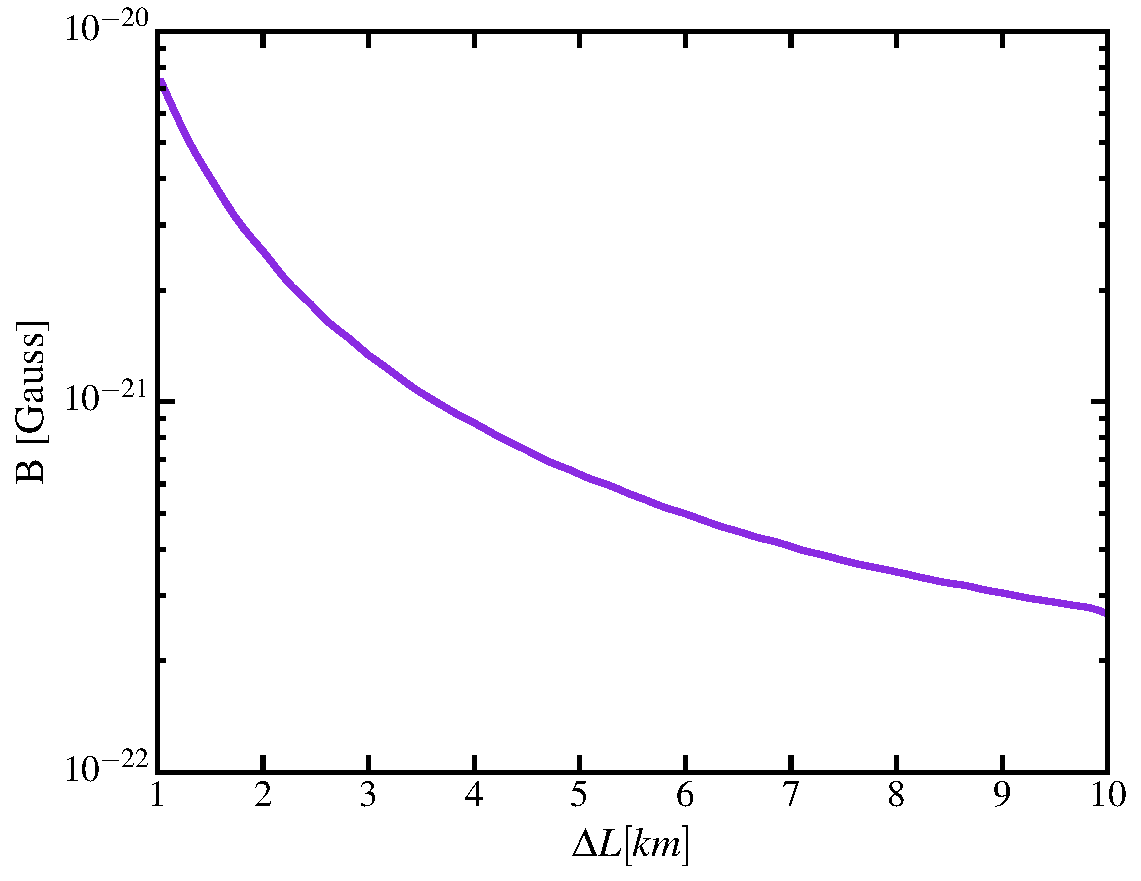
\includegraphics[width=.35\textwidth,keepaspectratio=true]{B0_vs_deltas.pdf}
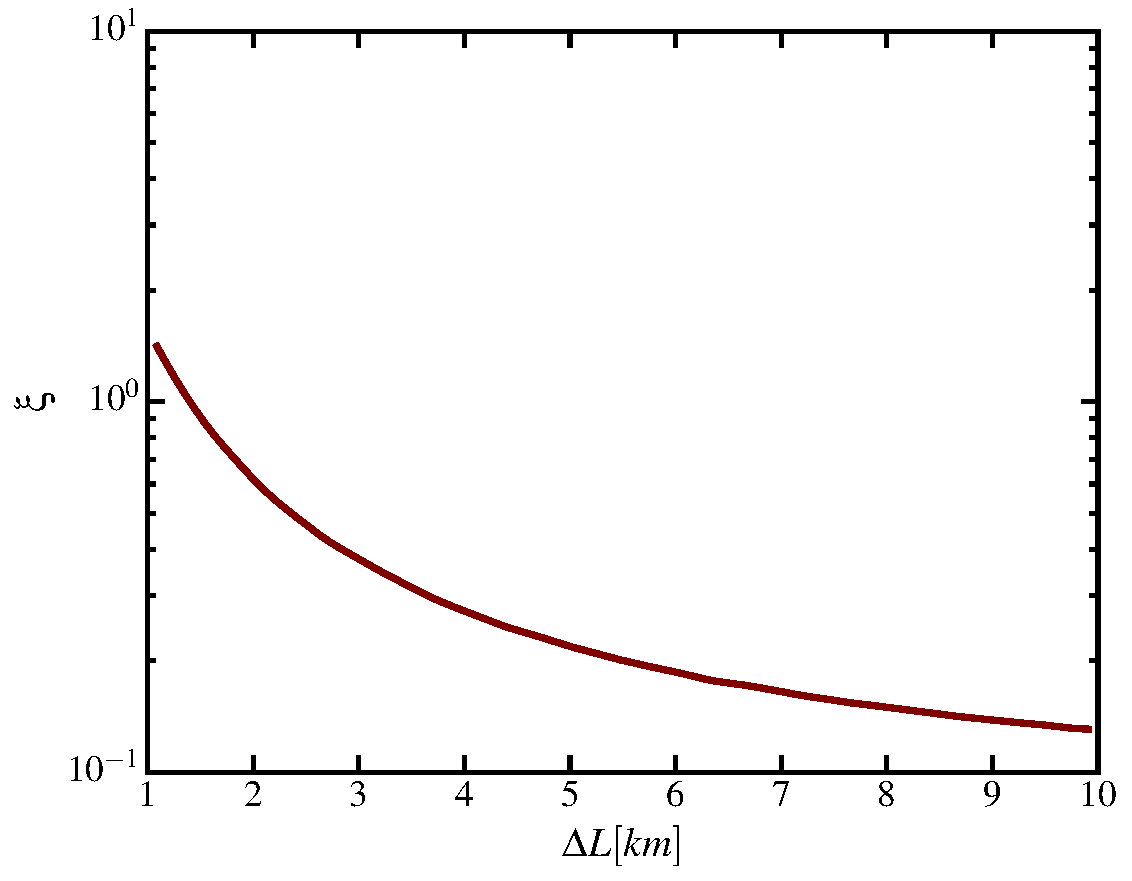
\includegraphics[width=.35\textwidth,keepaspectratio=true]{zeta_vs_deltas.pdf}
\caption{FFTT sensitivity to detecting a uniform magnetic field (left panel), and to distinguishing saturated case from no magnetic field (right panel), as a function of maximum baseline. Both are calculated for a survey size of 1 sr, assuming a uniform magnetic field in the entire survey volume.\label{fig:B0zeta_vs_deltas}}
\end{figure*}
%%%%%%%%%%%%%%%%%%%
\appendix
\section{Visibility-variance derivation}
\label{app_Vrms}

\begin{figure*}
\centering
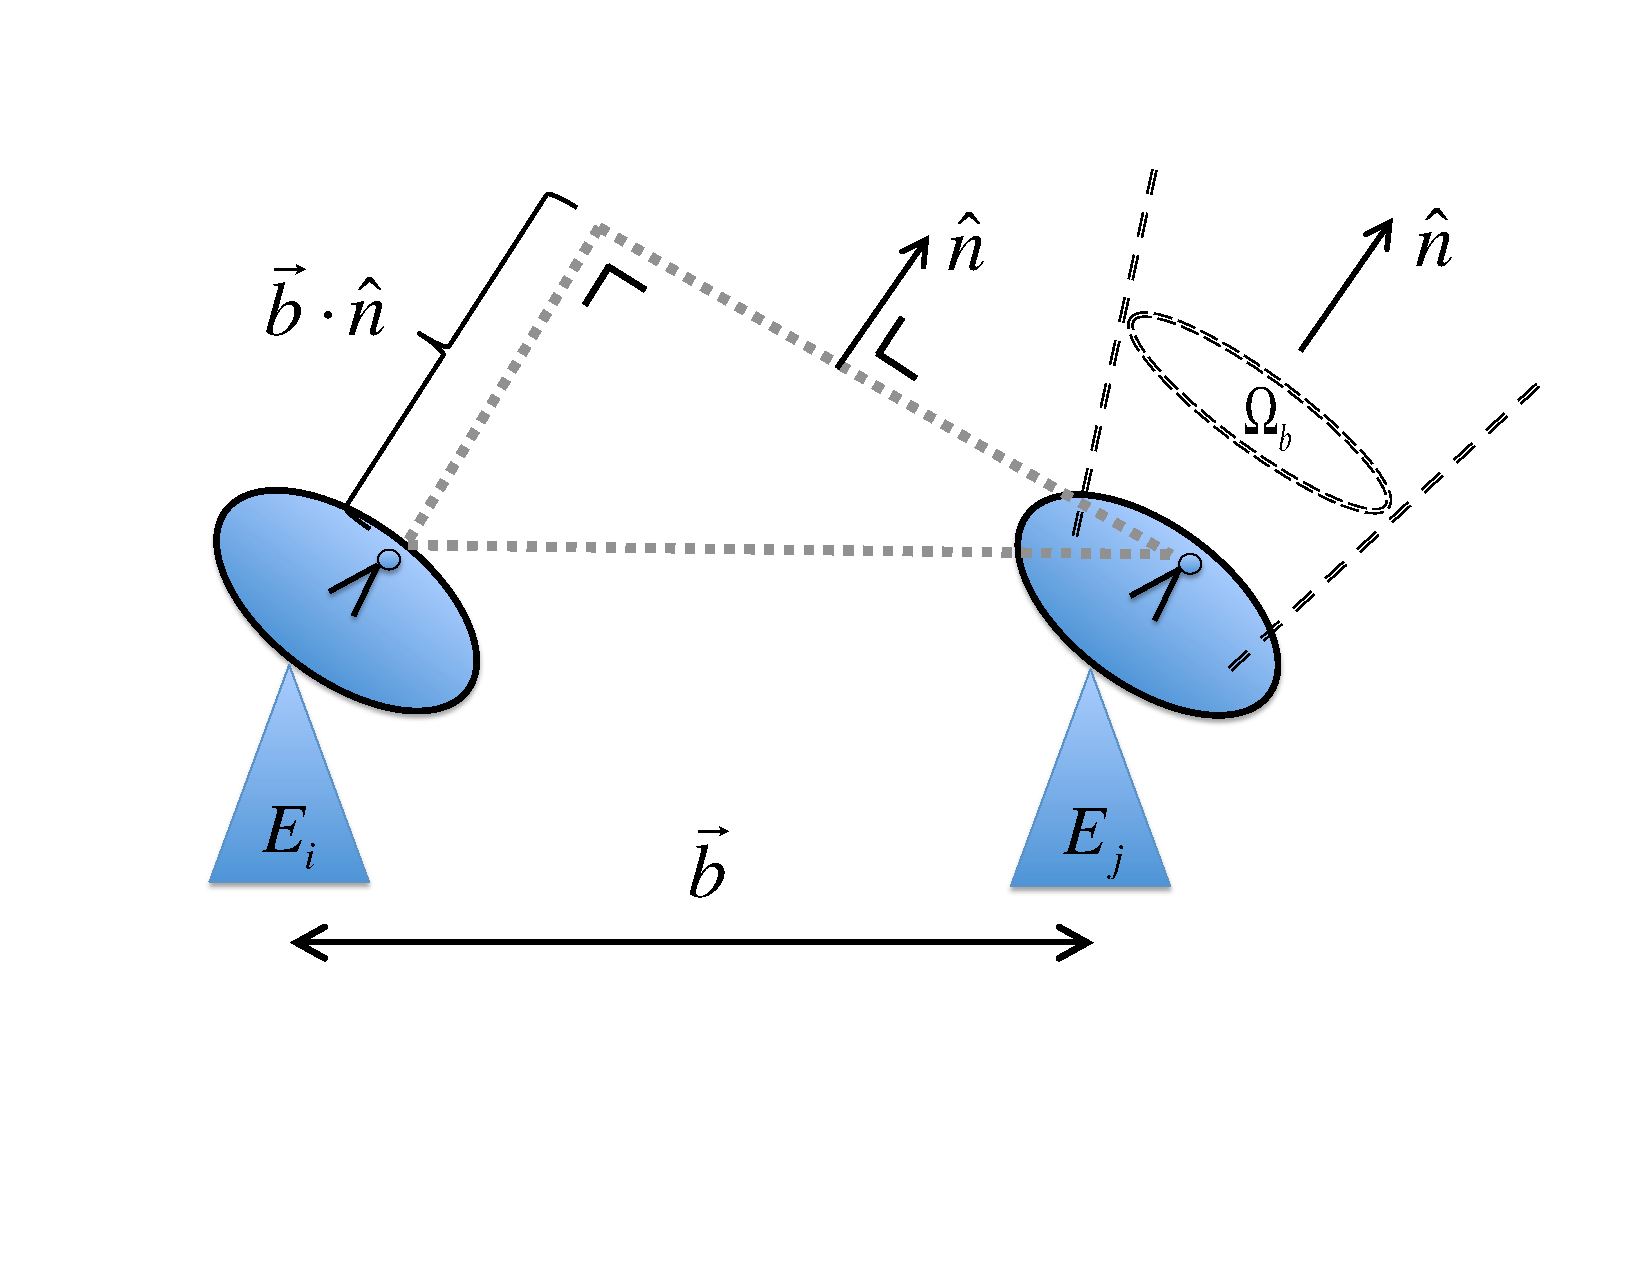
\includegraphics[width=.5\textwidth,keepaspectratio=true]{2antennae.pdf}
\caption{Two-antennae interferometer.\label{fig:2antennae}}
\end{figure*}

Here we derive the variance of the visibility for an interferometric array of two antennas separated by a baseline $\vec{b}$, each with an effective collecting area $A_e$, observing a single element in $uv$ plane for time duration $t_1$, in the total bandwidth $\Delta f = f_\text{max}-f_\text{min}$ of $N_f$ discrete frequencies. This setup is shown in Figure \ref{fig:2antennae}.

The quantity such interferometer measures is the correlation between electric fields $E_i$ and $E_j$ induced in the two antennae, as a function of the frequency. Since the observation time $t_1$ is finite, frequencies measured during $t_1$ are discrete, 
\beq
f_n = n/t_1, 
\label{eq:fn}
\eeq
where $n\in Z$, such that
\beq
E(t) = \sum_{n}\widetilde{E}(f_n)e^{2\pi if_nt}.
\eeq
The correlation coefficient of the electric fields is defined as
\beq
\rho_{ij}(f) \equiv \frac{\langle \widetilde{E}^*_i(f)\widetilde E_j(f)\rangle}{\sqrt{\langle |\widetilde{E}_i(f)|^2\rangle\langle|\widetilde E_j(f)|^2\rangle}},
\label{eq:rho_ij}
\eeq
for each measured frequency $f$. We now assume that $var(Re[ \widetilde E_i])=var(Im[\widetilde E_i])=\sigma^2$, such that the real (or imaginary) part of $\rho$ has the following variance
\beq
\bga
var(Re[\rho_{ij}(f)]) = \frac{1}{(2\sigma^2)^2}var(\langle Re[\widetilde{E}_i]Re[\widetilde{E}_j] + Im[\widetilde{E}_i]Im[\widetilde{E}_j]]\rangle) \\
= \frac{2\sigma^2\sigma^2}{(2\sigma^2)^2} = \frac{1}{2N_f} = \frac{1}{2t_1\Delta f},
\ega
\label{eq:var_Rerho}
\eeq
where the number of observed frequencies in time $t_1$ is derived from Eq.~\ref{eq:fn} to be,
\beq
N_f =  t_1\Delta f.
\label{eq:Nf}
\eeq

Before continuing, let us take a brief digression to show that the above formula implicitly assumes that the electric fields in the two antennas $\widetilde E_i$ and $\widetilde E_j$ have a very weak correlation, $\rho\ll 1$. Namely, suppose $x$ and $y$ are random Gaussian variables, where $var(x)\equiv\langle(x-\langle x\rangle)^2\rangle = \langle x^2\rangle - \langle x \rangle^2$, and similarly for $y$, and their correlation coefficient is $\rho\equiv \frac{\langle xy\rangle}{\sqrt{\langle x^2\rangle \langle y^2\rangle}}$. In this case, the following is true
\beq
\bga
var(xy) = \langle x^2y^2\rangle -  \langle xy \rangle^2 = 
\langle x^2\rangle \langle y^2\rangle + \langle xy\rangle^2\\
=\langle x^2\rangle \langle y^2\rangle+\rho \langle x\rangle^2\langle y\rangle^2=var(x)var(y)(1+\rho^2),
\ega
\eeq
so that when $\rho$ is small, then $var(xy)=var(x)var(y)$, which was assumed in the first equality of Eq.~\ref{eq:var_Rerho}.

Resuming the derivation, if different frequencies are uncorrelated, the result of Eq.~\ref{eq:var_Rerho} implies
\beq
\langle|\rho_{ij}(f)|^2\rangle = \frac{1}{t_1\Delta f}.
\label{eq:var_rho}
\eeq

The final step in this derivation requires the relation between intensity in the sky $\mathcal{I}(\vec\theta, f)$ (within the beam of size $\Omega_b$ in steradians) and the measured electric fields,
\beq
\langle \widetilde{E}_i^*(f)\widetilde{E}_j(f)\rangle = C \int_{\Omega_b} d^2\vec\theta\mathcal{I}(\vec\theta, f)e^{2\pi i\frac{ f}{c}\vec{b}_{ij}\cdot\vec{\theta}  }R(\vec\theta),
\label{eq:E_vs_mathcalI}
\eeq
where $\vec\theta=(\theta_x,\theta_y)$ is a unit vector that defines a direction in the sky, $C$ is a constant, and $R$ is the antenna response function (the shape of the beam in the sky); $\frac{2\pi f}{c}\vec{b}_{ij}\cdot\vec{\theta}$ is the phase delay between two antennae. From the above formula and Eq.~\ref{eq:rho_ij}, it follows\footnote{Note that a position in the $uv$ plane measures the phase lag between the two dishes in wavelenghts, such that $u\theta_x + v\theta_y\equiv\frac{\vec b\cdot \vec\theta}{\lambda}$.}
\beq
\rho_{ij}(f) = \frac{C\int_{\Omega_b}d^2\vec\theta\mathcal{I}(\vec\theta, f)e^{2\pi i(u\theta_x+v\theta_y)}}{C\int_{\Omega_b}d^2\vec\theta\mathcal{I}(\vec\theta, f)},
\label{eq:rho_mathcalI}
\eeq
where the denominator in the above formula approximately integrates to (for a small beam)
\beq
\int_{\Omega_b}d^2\vec\theta\mathcal{I}(\vec\theta, f) \approx
\Omega_b \mathcal{I}(\vec\theta, f).
\label{eq:rho_denominator}
\eeq
We can now use the approximate expression for the resolution of a single dish,
\beq
\Omega_b = \frac{\lambda^2}{A_e},
\label{eq:Omegab}
\eeq
the Reyliegh-Jeans law (or the definition of the brightness temperature),
\beq
\mathcal{I}(\vec\theta, f) = \frac{2k_BT_\text{sys}}{\lambda^2},
\label{eq:I_Tsys}
\eeq
and note that the numerator in Eq.~\ref{eq:rho_mathcalI} matches the definition of visibility (Eq.~\ref{eq:visibility}), to get 
\beq
\rho_{ij}(f) = \frac{A_e}{2k_BT\text{sys}}V(u,v,f),
\label{eq:rho_V}
\eeq
Substituting Eq.~\ref{eq:var_rho} into the above expression, we get the final result of this derivation,
\beq
\langle|V(u,v,f)|^2\rangle = \left(\frac{2k_BT_\text{sys}}{A_e\sqrt{t_1\Delta f}}\right)^2\delta(\vec{u}-\vec{u}')\delta_{ff'},
\label{eq:Vrms_final}
\eeq
where $V$ is a complex Gaussian variable, centered at zero, and uncorrelated for different values of its arguments.

It should be noted at the end that we were calculating the contribution to the visibility from the noise only (the system in the absence of a signal), so we used system temperature for brightness temperature (this could contain the signal from foregrounds and from the instrument). In case we want to repeat the computation in the presence of a signal, $T_\text{sys}$ should instead be the sum of the signal and the noise temperatures.

%What about polarization?
\appendix
\section{Integrand tests}
\label{tests}

\begin{figure*}[h]
\centering
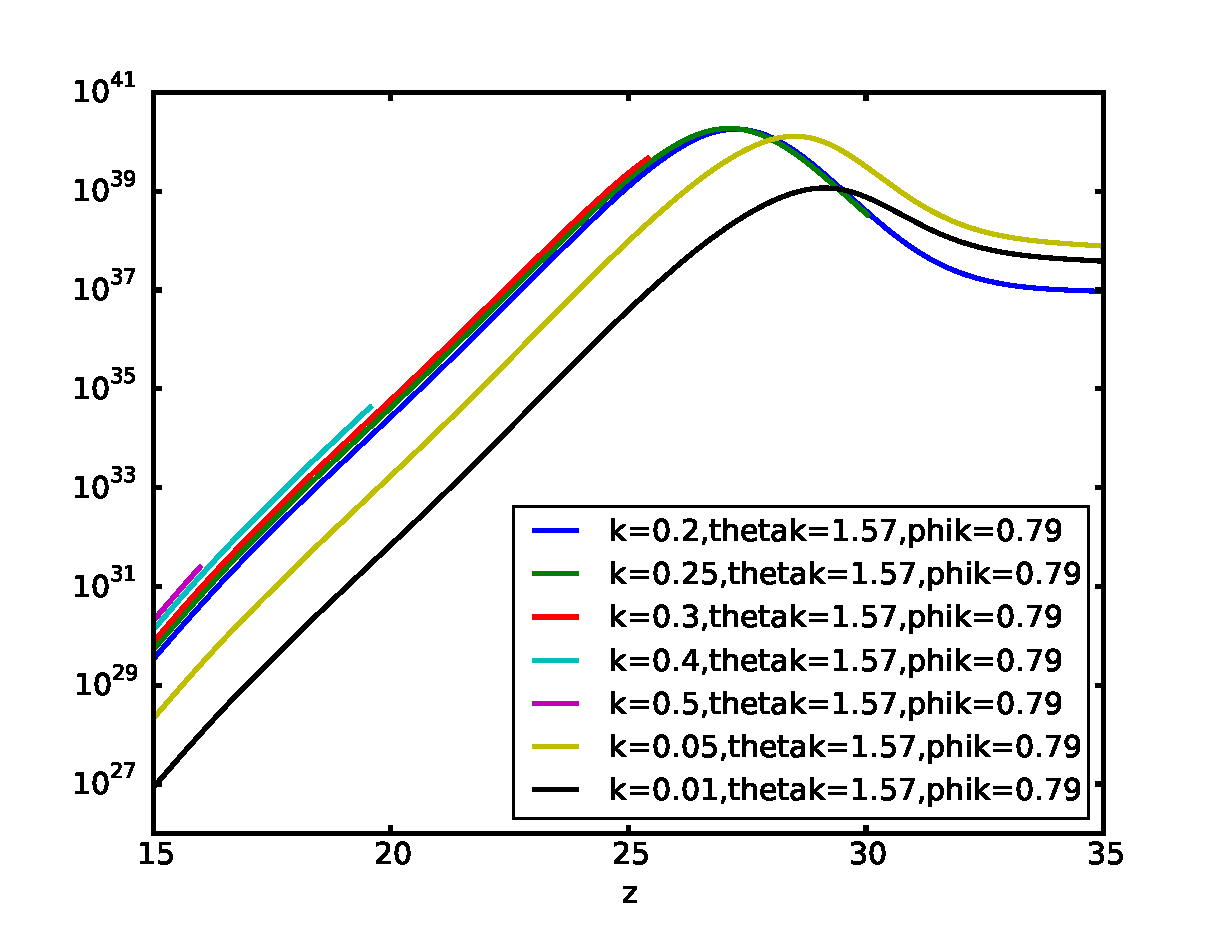
\includegraphics[width=.45\textwidth,keepaspectratio=true]{test_z.pdf}
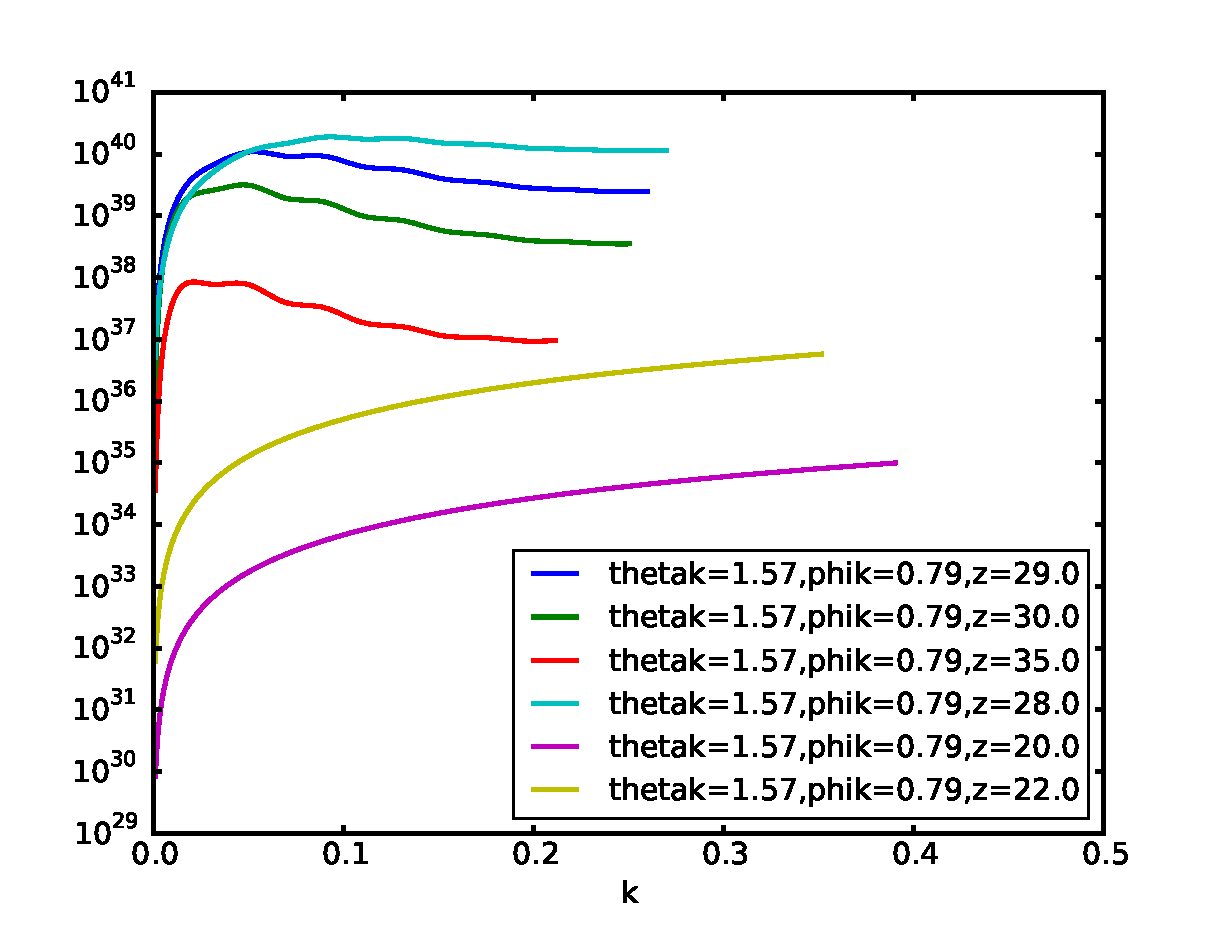
\includegraphics[width=.45\textwidth,keepaspectratio=true]{test_k.pdf}
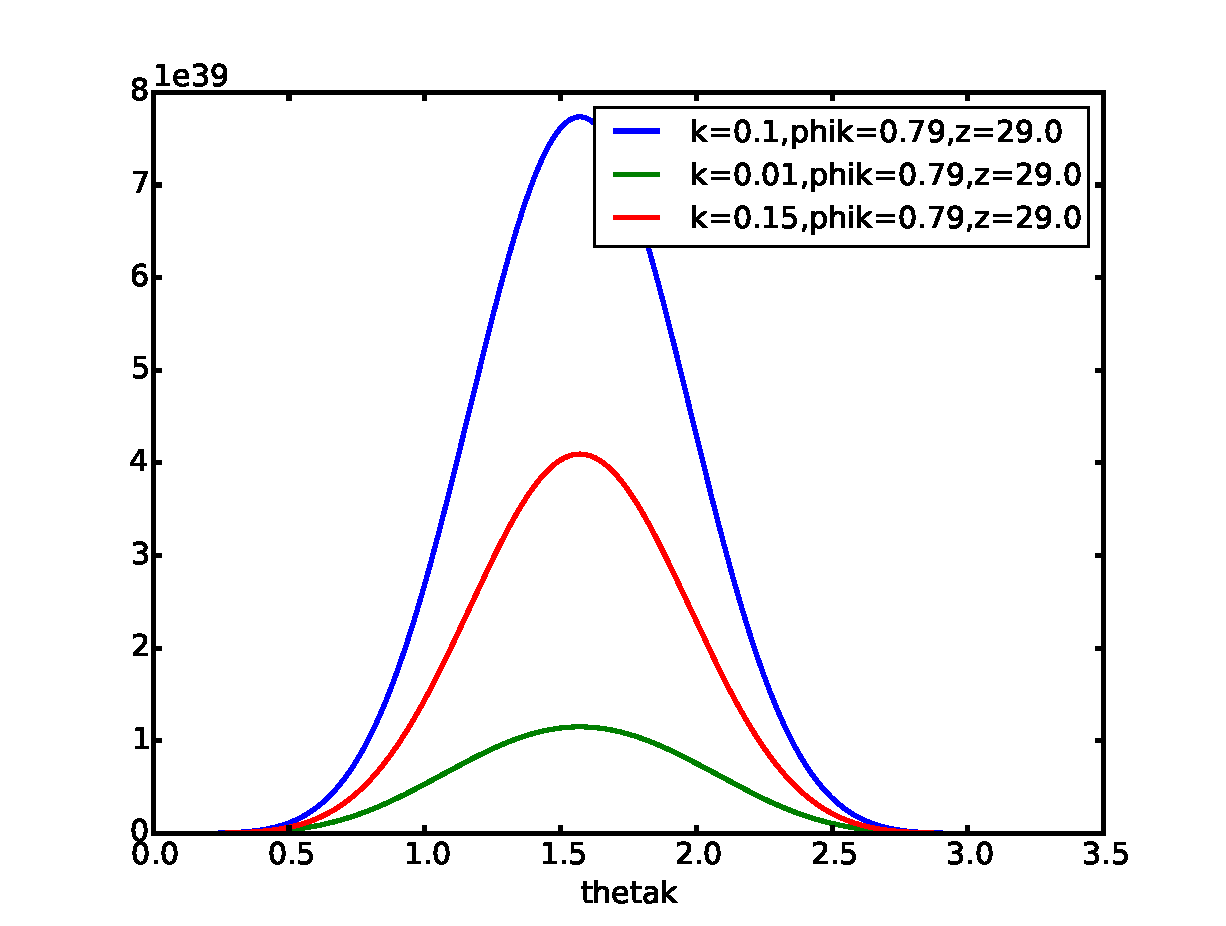
\includegraphics[width=.45\textwidth,keepaspectratio=true]{test_thetak.pdf}
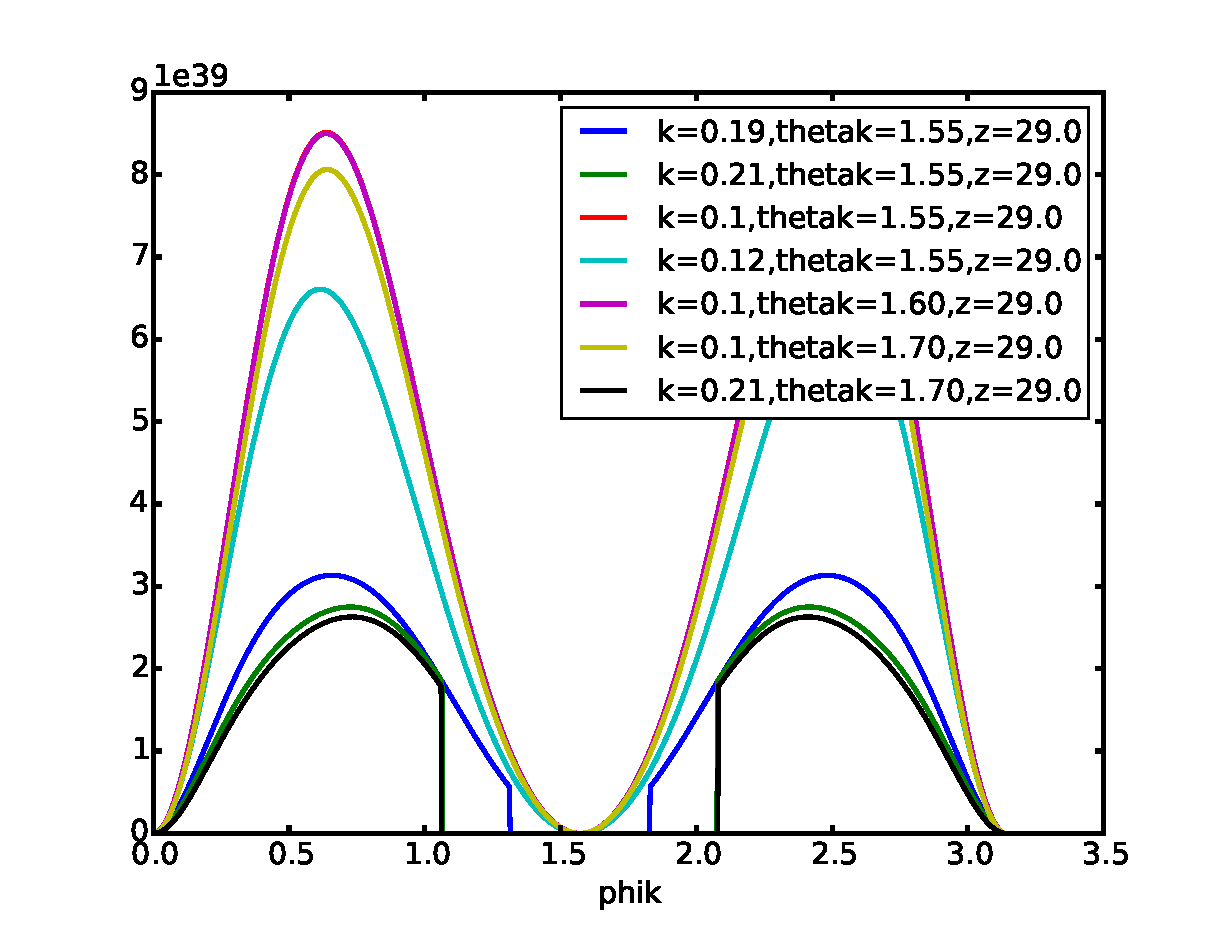
\includegraphics[width=.45\textwidth,keepaspectratio=true]{test_phik.pdf}
\caption{Slices through Fisher integrand for uniform B. Vertical axis is the value of individual summands in Eq.~\ref{eq:fisher_patch}.\label{fig:tests}}
\end{figure*}

\end{document}

